% Generated from frozen traces; keep titles and panel letters in LaTeX.
\providecommand{\TransientCaptionRevision}[1]{#1}
\begin{figure*}[t]
\centering
\subfloat[$v=13\,\mathrm{m/s}$\label{fig:oe-transient-v13}]{%
\begin{minipage}[t]{2.30in}
\centering
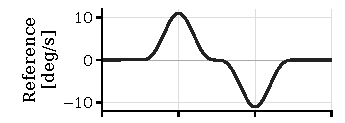
\includegraphics[width=\linewidth]{paper_oe_transient_compact_v13_reference_panel.pdf}\par\nointerlineskip
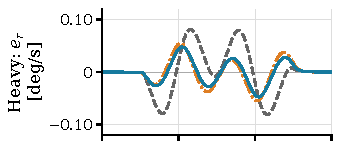
\includegraphics[width=\linewidth]{paper_oe_transient_compact_v13_heavy_panel.pdf}\par\nointerlineskip
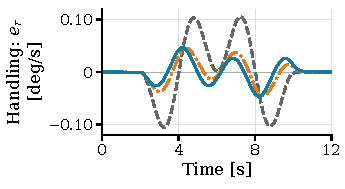
\includegraphics[width=\linewidth]{paper_oe_transient_compact_v13_handling_panel.pdf}\par\nointerlineskip
\end{minipage}}\hfill
\subfloat[$v=21\,\mathrm{m/s}$\label{fig:oe-transient-v21}]{%
\begin{minipage}[t]{2.30in}
\centering
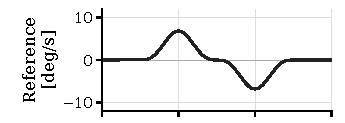
\includegraphics[width=\linewidth]{paper_oe_transient_compact_v21_reference_panel.pdf}\par\nointerlineskip
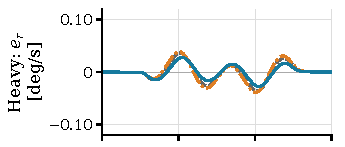
\includegraphics[width=\linewidth]{paper_oe_transient_compact_v21_heavy_panel.pdf}\par\nointerlineskip
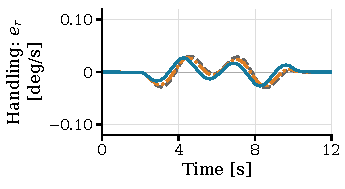
\includegraphics[width=\linewidth]{paper_oe_transient_compact_v21_handling_panel.pdf}\par\nointerlineskip
\end{minipage}}\hfill
\subfloat[$v=29\,\mathrm{m/s}$\label{fig:oe-transient-v29}]{%
\begin{minipage}[t]{2.30in}
\centering
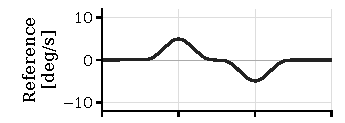
\includegraphics[width=\linewidth]{paper_oe_transient_compact_v29_reference_panel.pdf}\par\nointerlineskip
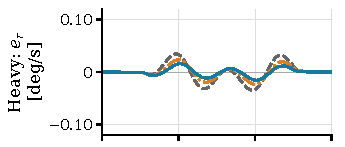
\includegraphics[width=\linewidth]{paper_oe_transient_compact_v29_heavy_panel.pdf}\par\nointerlineskip
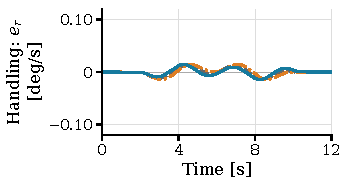
\includegraphics[width=\linewidth]{paper_oe_transient_compact_v29_handling_panel.pdf}\par\nointerlineskip
\end{minipage}}
\par\vspace{1pt}
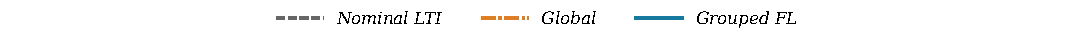
\includegraphics[width=\textwidth]{paper_oe_transient_compact_legend.pdf}
\caption{\TransientCaptionRevision{Fixed-speed yaw-rate tracking at three speeds unobserved in local identification. Top: reference $r_{\mathrm{ref}}$. Middle and bottom: errors $e_r=r-r_{\mathrm{ref}}$ for the same fixed heavy and handling recipients, respectively. All six error panels use identical limits. The reference has the same nominal lateral-acceleration demand at each speed.}}
\label{fig:oe-transient}
\end{figure*}
